\documentclass[a4paper, titlepage]{article}
\renewcommand{\baselinestretch}{1.15}				% line spacing 

% Package list
\usepackage{amsmath}
\usepackage[url=false, 
			sorting=none, 
			maxcitenames=2,
			hyperref=true]{biblatex}	% remove url visit date and sort references by appearance
\usepackage{hyperref}
\usepackage{helvet}									% helvetica font
\usepackage{rotating}
\usepackage{array}
\usepackage{multirow}
\newcolumntype{C}[1]{>{\centering\arraybackslash}p{#1}}

\renewcommand{\thefootnote}{\alph{footnote}}
% Biblatex configuration
\addbibresource{library.bib}
\DeclareNameAlias{author}{family-given}

% ideas for paper
% add carbon taxes
% add ports as possible sinks
% add eucalyptus
% add electrolysis


\begin{document}
\title{Paper title}
\author{
	Diego Lopes\\
	\and
	Moisés Teles dos Santos}
\date{01/07/2025}
\maketitle

\begin{abstract}
	This is the papers abstract, version 2!
\end{abstract}

\section{Introduction}

Since 1961, worldwide food supply per capita has raised by 30\%, in large part because of the increase of use of
nitrogen fertilizers to improve agricultural productivity \cite{mbowIPCCSpecialReport2019}. The importance of
fertilizers on agriculture cannot be overstated, with research indicating that half of the world’s population
is sustained by mineral fertilizers. The agricultural sector is also responsible for between 11\% and 15\% of
all greenhouse gas (GHG) emissions worldwide \cite{ifaEstimatingReportingFertilizerRelated2016}, with fertilizers
accounting for 2\% to 3\% of emissions \cite{brentrupCarbonFootprintAnalysis2016}. Production of mineral fertilizers
is dependent on fossil fuels and raw materials, including mineral extraction,
transportation, manufacturing, and power supply. In this scenario, decarbonizing the fertilizer sector is equally
important to the industry’s expansion \cite{ouikhalfanNetZeroEmissionFertilizers2022}, considering the GHG emissions
reduction preconized in the Paris agreement (2015).

The mineral fertilizers divide themselves into three main categories, each one corresponding to the main
macronutrient present in its composition: nitrogen (N), phosphorus (P) and potassium (K). Although none of the
macronutrients can be considered more or less important than the other, nitrogen is the one consumed at higher
volumes, and also the one with the more energetically intensive manufacturing
process \cite{ieaAmmoniaTechnologyRoadmap2021}. Out of all nitrogen fertilizers, urea is the main commercial product,
with ammonia as its obligatory precursor. Ammonia ($NH_3$) is obtained by the synthesis of hydrogen ($H_2$)
and nitrogen $N_2$ through the traditional Haber-Bosch process, responsible for the production of more than 90\% of
worldwide ammonia \cite{applAmmoniaPrinciplesIndustrial1999}. Nitrogen is obtained from the atmosphere,
but hydrogen is traditionally obtained from steam reforming of fossil fuels; 72\% of the worldwide ammonia
production comes from natural gas reforming, while 26\% is obtained from coal gasification. 1\% is produced
through other petroleum derivatives, while the renewable fraction, produced through water electrolysis,
corresponds to less than 1\% \cite{ieaAmmoniaTechnologyRoadmap2021}. Urea, in turn, is produced by the Basarov reaction
using ammonia and carbon dioxide ($CO_2$), with this process being responsible for all commercial urea production
in a large scale \cite{meessenUrea2010}. The $CO_2$ is supplied by the reforming syngas, as both $CO$ and $CO_2$ must
be removed prior to the ammonia synthesis as they are poisons to the commercial catalysts.

Since both processes are energetically intensive, efforts were made throughout the 20\textsuperscript{th} century to
improve its energy efficiency, involving equipment changes, process control and residual heat utilization. With these
efforts, current ammonia production is very close to the theoretical minimum energy consumption
\cite{ieaAmmoniaTechnologyRoadmap2021}.
Considering the small efficiency improvements still possible, a natural future step is to search for sustainable
replacements for the process’ feedstocks and energy usages.

In this scenario, biomass is a promising feedstock replacement. Among the conversion routes, gasification is of special
interest considering that the biomass syngas composition is similar to the fossil fuel syngas obtained in traditional
processes; in that sense the conversion technologies of this syngas into alcohols, hydrocarbons and other chemicals
can be leveraged with significant overlap. Despite that, biorefineries pose additional challenges to the conventional
plants. Given its high volume and low energetic density compared to fossil fuels, the feasibility of all biorefineries
depend heavily on the local availability of biomass inputs and spatial allocation of this biomass
. This demonstrates the need for an integrated approach in biorefinery
modeling that combines technical performance, location, capacity and configuration of the plant
\cite{schroderImprovingBiorefineryPlanning2018}.

\section{Literature Review}

The mathematical modeling of biomass gasification, ammonia, urea and its subprocesses has been the object of multiple
studies. \textcite{baruahModelingBiomassGasification2014} presented a systematic review of  existing techniques to model
biomass gasification systems, categorized by gasifier type, feedstock and parameters studied,
concluding that equilibrium modeling is the most suitable technique for process studies on the influence of fuel and
process parameters, since these models are independent of gasifier's design.
\textcite{gambarottaNonstoichiometricEquilibriumModel2018} and \textcite{azzoneDevelopmentEquilibriumModel2012} developed
equilibrium models for biomass gasification and compared the model’s results against experimental data, predicting the
syngas composition with reasonable accuracy. Gasification models were successfully implemented in commercial process
simulators such as Aspen Plus, in \textcite{hanModelingDowndraftBiomass2017} and
\textcite{ramzanSimulationHybridBiomass2011}

The ammonia synthesis process has also been modeled extensively. The reaction mechanisms and kinetics have been
studied since the 1930s \cite{gillespieThermodynamicTreatmentChemical1930} and the Temkin-Pyzhev formulation is
used to this day in ammonia reactor designs \cite{temkinKineticsAmmoniaSynthesis1940}
\cite{singhSimulationAmmoniaSynthesis1979} \cite{nielsenAmmoniaCatalysisManufacture1995}.
\textcite{florez-orregoProcessSynthesisOptimization2018} has modeled the full fossil fuel process and conducted
exergy analysis and optimization while \textcite{domingosExergyEnvironmentalAnalysis2021} has applied the same model
for ammonia production through black liquor gasification, with promising results reaching negative emissions in
certain scenarios. Ammonia production via other biomasses have also been proposed by
\textcite{florez-orregoComparativeExergyEconomic2019} and \textcite{tunaTechnoeconomicAssessmentNonfossil2014}, with
both studies identifying substantial environmental benefits in using biomass as a feedstock, despite a lower energy
efficiency in the process.

The urea process is also studied since the start of the 20\textsuperscript{th} century, with early works on the
urea synthesis published by \textcite{frejacquesBasesTheoriquesSynthese1948} and
\textcite{kawasumiEquilibriumCO2NH3UreaH2OSystem1953}, and \textcite{islaSimulationUreaSynthesis1993}, all focusing
on describing and modeling the complex thermodynamics in the urea reactor. Despite this, more extensive models of
the full process are far rarer, as are attempts at optimizing it.
\textcite{meessenUreaSynthesis2014} describes the main commercial processes available in the industry, and
\textcite{aspentechASPEN88Technical2011} published a process model for the urea synthesis loop based on the
Stamicarbon stripping process. Given the difficulties in predicting the urea $NH_3$-$CO_2$-water equilibrium, this
model has been leveraged directly by several authors.

\textcite{zhangTechnoeconomicComparison1002021} presented process models for the full gasification, ammonia and urea
process with the traditional fossil fuel route and two renewable alternatives, using biomass gasification and water
electrolysis. \textcite{alfianMultiobjectiveOptimizationGreen2019} also modeled the same systems and used a
multi-objective optimization model to select the technology that minimizes production costs and environmental impact.
\textcite{domingosExergyEnvironmentalAnalysis2021} evaluated the production of urea via black liquor gasification
and \textcite{gyanwaliTechnoeconomicAssessmentGreen2023} assessed the renewable urea production utilizing solid waste
and power as feedstocks.

% TODO: LITERATURE REVIEW ON SUPPLY CHAIN OPTIMIZATION
Parallel to the physico-chemical modeling of the process, modeling frameworks that incorporate optimization of
supply-chain aspects and plant location have been gaining increased attention.
\textcite{dunnettSpatiallyExplicitWholesystem2008} proposed a combined production and logistics model, formulated as a
mixed-integer linear programming (MILP) model , for the lignocellulosic ethanol production in a hypothetical geographical
area composed of a 5x5 grid and found out that the optimal production costs are highly sensitive to the spatial
distribution of biomass. \textcite{kimDesignBiomassProcessing2011} developed a MILP model for the production of bio-gasoline and
biodiesel from forestry residues that incorporates the selection of technology, capacity and biomass location into the
decision making. \textcite{schroderImprovingBiorefineryPlanning2018} implemented a combined model for a synthesis
gas biorefinery producing multiple products and used a non-linear approach coupled with an evolutionary algorithm to
determine an optimal approach in terms of location and products produced. \textcite{theozzoMILPFrameworkOptimal2021}
proposed an optimization framework for forestry products that considers not only the biomass and plant locations,
but also the storage and market layers, with his model also leveraging forestry dynamics and seasonality.

Despite these multiple works, there's still much room for improvement. While the influence of gasification parameters
on the syngas composition is well-known from gasification models and previous works, it is unclear how these
composition differences affect the performance and profitability of the urea plant as a whole, given that all studies
consider only one combination of gasifying agent and biomass. A scenario evaluation comparing the plants’ key
performance indicators (KPIs) with different biomasses and gasification conditions is therefore critical in
understanding the feasibility of renewable urea production, as is the comparison of the renewable plant with
actual process data from existing state-of-the-art urea plants.

The published process models could also be improved. Commercial urea is traditionally marketed in its granulated or prilled
form with 99 wt.\%+ purity, and all published studies deliver urea in a lower concentration, closer to 77 wt.\%,
corresponding to the concentration on the outlet of the distillation unit. The urea evaporation and condensate
treatment are energy intensive, and the recovery of ammonia dissolved in the liquid urea can improve the yield of the
process significantly \cite{meessenUreaSynthesis2014}, while other improvements such as hydrogen recovery from the
necessary ammonia purge gas are absent in recent literature. The urea process also offers interesting opportunities
in heat recovery, given that the high-pressure carbamate condenser rejects a large amount of heat at medium
temperatures, and how to maximize this heat integration is unclear since in all studies published the heat exchanger
network and utilities are abstracted from the final process model.

Finally, none of the proposed models for renewable urea production consider the biomass logistics, supply-chain and
distribution of the final product. In the case of using agricultural wastes as the feedstock, this is even more
important considering the evident synergy between receiving waste and providing fertilizer to the same locations.

\section{Methodology}

In this section a complete description of the process models, optimization model and methodology will be presented.
The process models were developed on commercial software Aspen Plus v8.8. Aspen Energy Analyzer was used to evaluate
the heat exchanger network and propose the utilities integration.

For the optimization model, a Python application was developed, with Pyomo was chosen as the modeling language. The
commercial solver Gurobi was used to solve the model. Financial and environmental calculations were made in
Microsoft Excel.

\subsection{Process Model}

\subsubsection{Biomass Gasification}

A process flow diagram of the gasification process is presented in \autoref{img_aspengasification}. Biomass was modeled
in Aspen Plus as a non-conventional component. \autoref{tab_biomass} presents the composition and heating value
of the main biomasses studied. 

\begin{figure}
	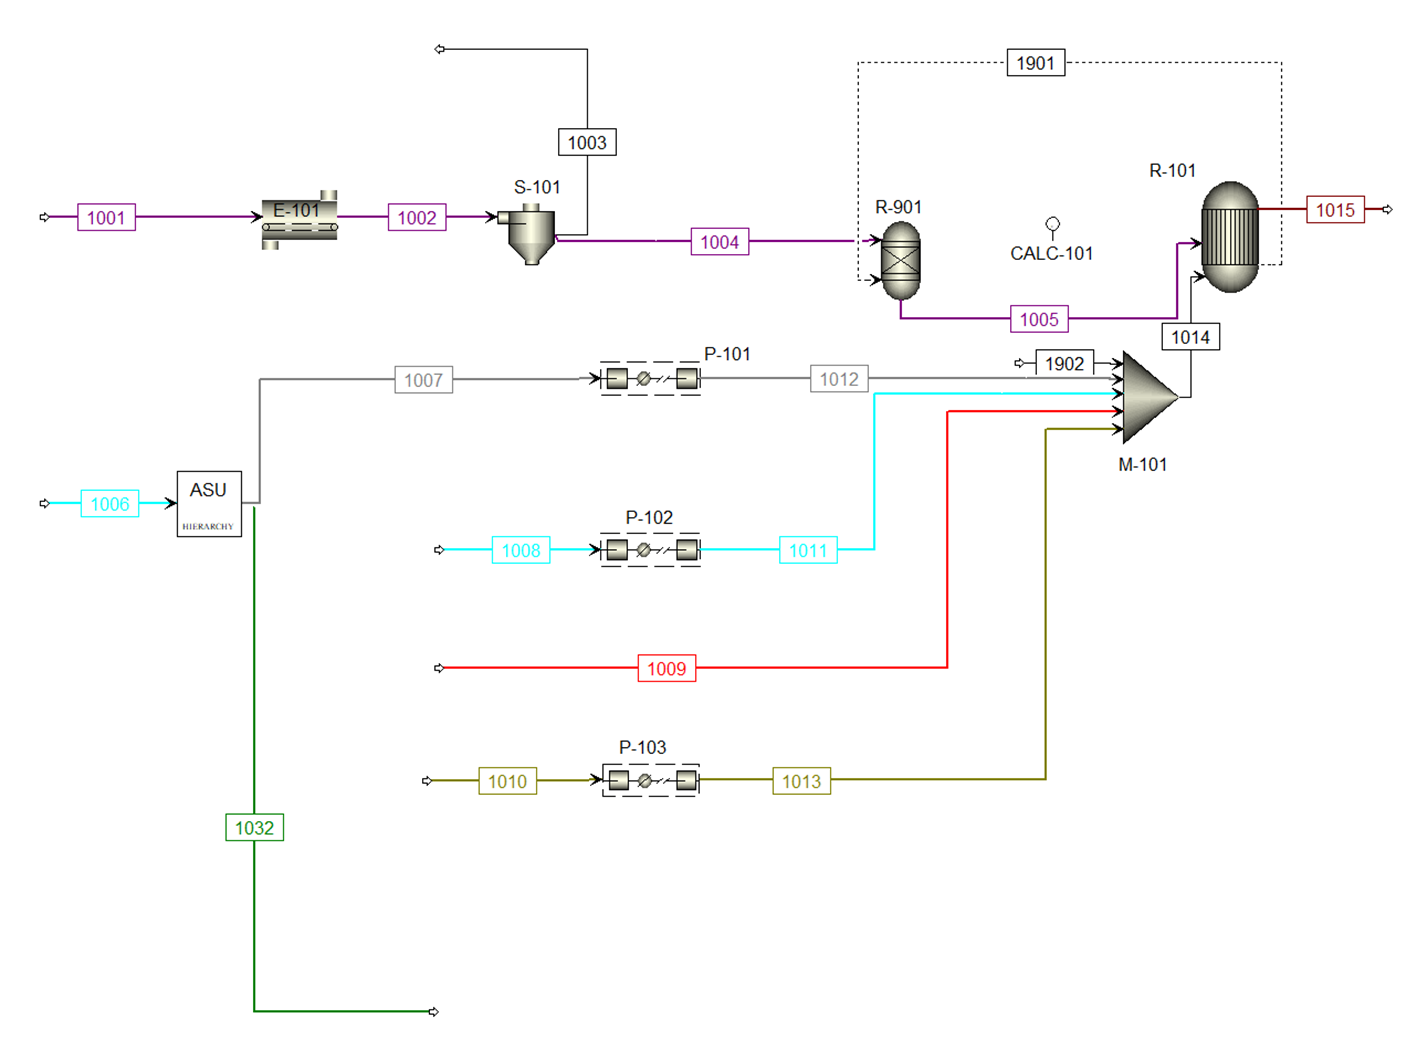
\includegraphics[width=\textwidth]{img/aspen_gasification.png}
	\caption{Biomass gasification process flow diagram}
	\label{img_aspengasification}
\end{figure}

\begin{sidewaystable}
	\caption{Biomass data}
	\label{tab_biomass}
	\begin{tabular}{||c | c | C{2.0cm} | C{2.0cm} | C{2.0cm} | C{2.0cm} | C{2.0cm} | C{2.0cm} ||}
		\hline
		 & & \multicolumn{6}{c||}{Biomass} \\
		\hline
		Name & Unit & Sugarcane bagasse \cite{jorapurSugarcaneLeafbagasseGasifiers1997} & Sugarcane straw \cite{jorapurSugarcaneLeafbagasseGasifiers1997} & Soybean straw \cite{tahirCatalyticFastPyrolysis2021} & Corn \cite{evansDevelopmentBiomassGasification1988} & Rice \cite{gaurAtlasThermalData1995} & Coffee \cite{anggonoCharacteristicsBiomassBriquettes2023} \\
		\hline
		Moisture & kg/kg \footnotemark[1] & 0.4000 & 0.2000 & 0.2000 & 0.2000 & 0.2000 & 0.2000 \\
		Ash & kg/kg \footnotemark[1]& 0.0420 & 0.0770 & 0.0530 & 0.0735 & 0.1580 & 0.0587 \\
		\hline
		C & kg/kg daf \footnotemark[2] & 0.4703 & 0.4312 & 0.5432 & 0.5025 & 0.4628 & 0.5221 \\
		H & kg/kg daf \footnotemark[2] & 0.0561 & 0.0596 & 0.0544 & 0.0628 & 0.0607 & 0.0569 \\
		O & kg/kg daf \footnotemark[2] & 0.4735 & 0.5071 & 0.3761 & 0.4287 & 0.4506 & 0.4066 \\
		N & kg/kg daf \footnotemark[2] & 0.0000 & 0.0021 & 0.0262 & 0.0060 & 0.0258 & 0.0143 \\
		\hline
		HHV & kJ/kg daf \footnotemark[2] & 18557 & 17430 & 18230 & 20500 & 18610 & 18795 \\
		\hline
	\end{tabular}

	\footnotetext[1]{As received}
	\footnotetext[2]{Dry and ash free}
\end{sidewaystable}
Biomass (1001) is received and dried to 15\% moisture in dryer E-101 by using low-pressure steam from the utilities
plant. 
Ash is separated at the solids separator and the biomass is converted from non-conventional into conventional 
components ($C$, $H_2$, $O_2$, $N_2$, $H_2O$) in a yield reactor (RYield) by using a calculator block. 
The decomposed biomass is mixed with the gasifying agents (pure oxygen, air, high-pressure steam and $CO_2$,
represented by streams 1007, 1008, 1009 and 1010, respectively) and gasified in the Gibbs reactor R-101.
Pure oxygen is supplied by the air separation unit, while $CO_2$ is supplied by the carbon capture system.

The gasification occurs on an entrained-flow gasifier, modeled using a non-stoichiometric equilibrium approach, 
due to its flexibility for comparing biomasses with different compositions 
\cite{gambarottaNonstoichiometricEquilibriumModel2018}. A global gasification reaction can be described as:

\begin{multline}
	CH_aO_bN_c + wH_2O_{(l)} + sH_2O_{(g)} + e(O_2+\rho N_2) + dCO_2 \rightleftharpoons n_{CH_4}CH_4 \\ 
	+ n_{CO_2}CO_2 + n_{CO}CO + n_{H_2}H_2 n_{H_2O}H_2O + n_{O_2}O_2 + n_{N_2}N_2
\end{multline}

With $a$, $b$ and $c$ being derived from the biomass composition; $w$, $s$, $e$, $\rho$ and $d$ representing the
gasifying agent mixture, and $n_i$ being the number of moles of component $i$ in the syngas. At equilibrium, the Gibbs
energy of the mixture ($G$) must be at minimum.

\begin{equation}
	G = \sum_{i=1}^{M}{n_iG_i^0} + \sum_{i=1}^{M}{n_iRT ln \left( \frac{n_i}{n_{tot}} \right) }
\end{equation}

The number of moles of each component, $n_i$, are constrained by the mole balance of each atom C, H, O and N on the
biomass. Tar formation is not considered in this model. The minimization of Gibbs energy is obtained on the Gibbs 
reactor block (RGibbs). Syngas properties were calculated using the Peng-Robinson equation of state, 
with Boston-Mathias modifications. The gasification conditions are initially set to 30 bar of pressure and a 
temperature of 1200°C.  The temperature is controlled by the oxygen injection on the gasifier. All other gasifying 
agents are parameters of the model.

\subsubsection{Air separation unit}

A process flow diagram of the air separation unit is presented in \autoref{img_aspenasu}. 
Air is compressed in a multistage compressor (P-501) to an intermediate pressure of 6 bar and split into 2 streams. 
One stream (5003) is further compressed in compressor P-502 to a higher pressure of 7.5 bar and liquefied in a 
multi-stream heat exchanger using the products from the distillation section. 
The lower pressure air stream (5010) is cooled in the same heat exchanger and used as the vapor feed for the 
high-pressure column operating at 6 bar.
A rich nitrogen stream is removed as the distillate fraction from the HP column (5014), while the bottom fraction is 
a rich oxygen mixture (5015). 
Both streams are further cooled in a second multi-stream heat exchanger and sent to the low-pressure column operating
at 1.8 bar for further separation. The rich nitrogen fraction is fed at the top of the column while the rich oxygen 
fraction is fed at an intermediate stage. The columns are thermally coupled in the sense that the reboiler duty of the
low-pressure section is the condenser duty from the high-pressure section, and the liquified air expansion is the 
thermal drive for the separation.

The system is designed to produce $N_2$ with 99.5\% mole fraction and $O_2$ with 99\% mole fraction. These purities
are achieved by manipulating the high-pressure/low-pressure split at S-501, and the high-pressure column 
reflux ratio in design specifications. The $O_2$ is sent directly to the gasification system, while the $N_2$ is 
partially sent to the ammonia synthesis unit while the excess is compressed and sold as a separate product.

\begin{figure}
	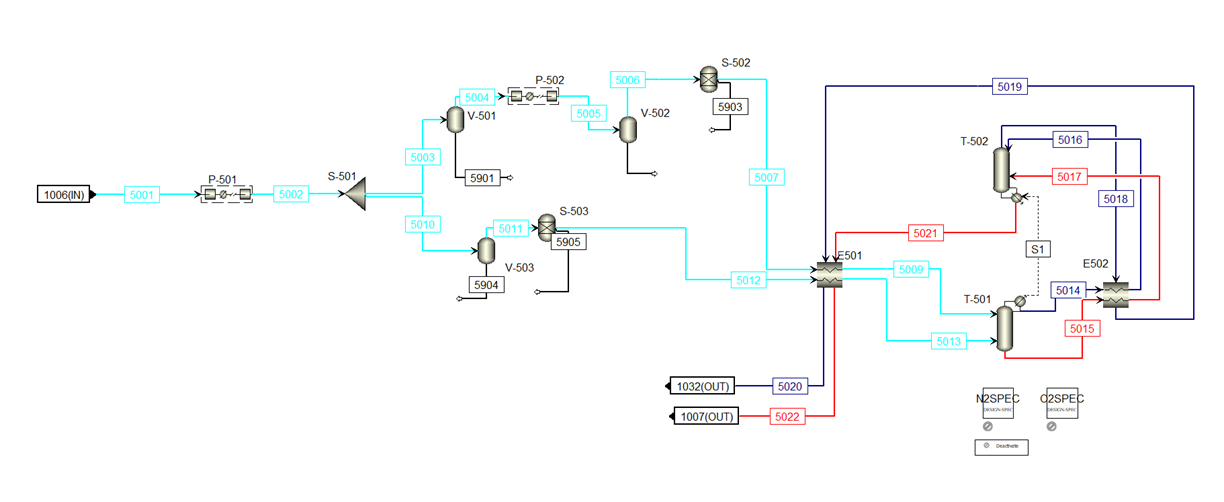
\includegraphics[width=\textwidth]{img/aspen_asu.png}
	\caption{Air separation unit (ASU) process flow diagram}
	\label{img_aspenasu}
\end{figure}

\subsubsection{Gas Conditioning}

A process flow diagram of the gas conditioning unit is presented in \autoref{img_aspenconditioning}

\begin{figure}
	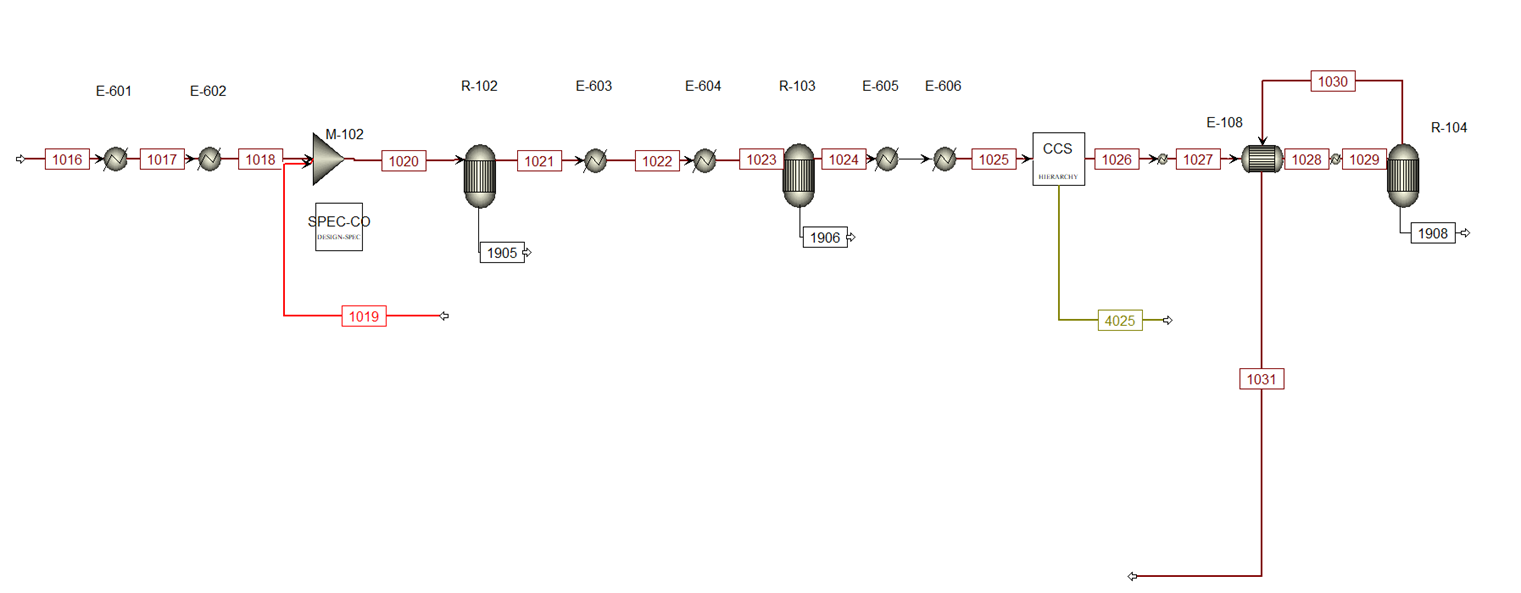
\includegraphics[width=\textwidth]{img/aspen_conditioning.png}
	\caption{Gas conditioning unit process flow diagram}
	\label{img_aspenconditioning}
\end{figure}

The syngas from the gasification plant is rich in both $H_2$ and $CO$. Given that $CO$ is undesired in the 
ammonia synthesis, a gas conditioning unit is designed to maximize the $H_2$ concentration on the syngas by leveraging 
the water-gas shift reaction. This reaction can be described as:

\begin{equation}
	CO + H_2O \rightleftharpoons CO_2 + H_2 \quad \Delta H_{ref}^0 = -41 kJ/mol
\end{equation}

The water-gas shift reaction is exothermic and driven by equilibrium, which means that low temperatures favor the
product formation. At the same time, the reaction kinetics is favorable in high temperature, which means that there's 
a tradeoff between $CO$ conversion and reactor size \cite{florez-orregoProcessSynthesisOptimization2018}. Therefore, 
the chosen design uses two shift reactors operating with inlet conditions of 310°C and 210°C, and intermediate cooling.

The hot syngas from the gasification section (1016) is cooled to 310°C in two utility heat exchangers
(E-602 and E-603), generating high pressure superheated steam. The syngas is then mixed with high pressure steam 
(1019) produced in the utility unit and sent to the high temperature shift reactor (R-102). The partially shifted 
syngas is cooled to 210°C into 2 intermediate heat exchangers (E-603 and E-604), also connected to the utilities 
plant, and sent to the low temperature shift reactor (R-103) for further $H_2$ generation. The syngas is cooled yet 
again at 2 utility heat exchangers (E-605 and E-606), to maximize the heat recovery of the process.

The $CO_2$ on the syngas (4025) is captured at the carbon capture and storage (CCS) unit, described in the next 
section. After the $CO_2$ capturing, the final step in the gas conditioning is to remove any remaining $CO$ and $CO_2$
in the syngas, considering that both molecules are poisons to the ammonia catalysts. This is done in a methanation 
reactor (R-104). The methanation reaction is also equilibrium-driven and can be described as:
\begin{alignat}{2}
	&CO + 3H_2 \rightleftharpoons CH_4 + 3H_2O \quad & &\Delta H_{ref}^0 = -206 kJ/mol \\
	&CO_2 + 4H_2 \rightleftharpoons CH_4 + 4H_2O \quad & &\Delta H_{ref}^0 = -164 kJ/mol
\end{alignat}


These reactions consume $H_2$ and generate $CH_4$, which is an inert on the ammonia loop. Therefore, they are undesired 
for the process.

The steam injection at the start of the process is a design specification of the model and is set to control the mole
fraction of $CO$ at the CCS inlet (1025) to below 0.5\%. Syngas properties for this unit were calculated using 
the Peng-Robinson equation of state, with Boston-Mathias modifications.

\subsubsection{Carbon capture}

A process flow diagram of the carbon capture and storage unit is presented in \autoref{img_aspenccs}.
A physical absorption system using DEPG (dimethyl ethers of polyethylene  glycol) was chosen for this step, widely
used for $CO_2$ capture in gasification for syngas production. The proposed system is based on the optimized design
of \textcite{martelliMultiobjectiveOptimizationSelexol2015} and modified for the biomass gasification specific needs. 

\begin{figure}
	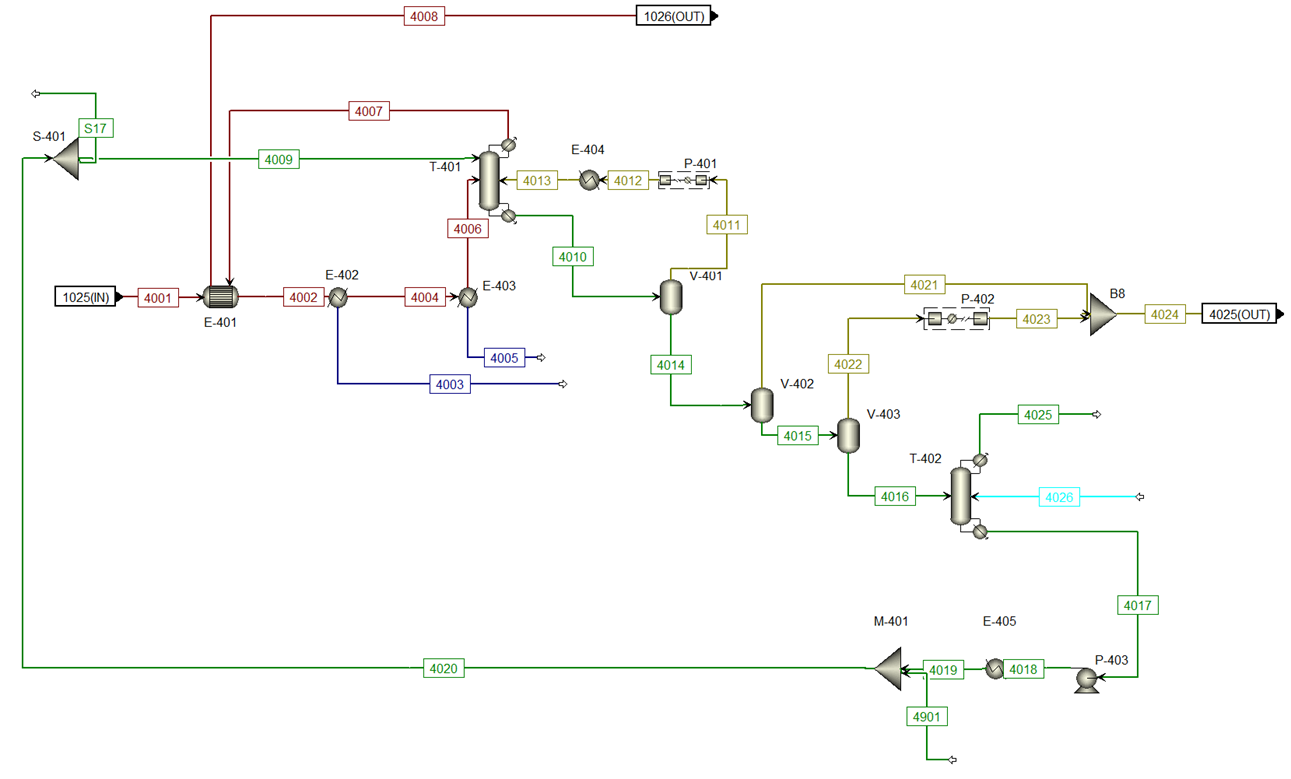
\includegraphics[width=\textwidth]{img/aspen_ccs.png}
	\caption{Carbon capture unit process flow diagram}
	\label{img_aspenccs}
\end{figure}

The syngas (4001) at 30 bar is cooled to 4°C in 3 stages by using purified syngas (E-401), cooling water (E-402) and
chiller water (E-403) and sent to the absorber column (T-401) where it gets in contact with the $CO_2$-lean 
solvent (4009). The $CO_2$ on the rich solvent (4010) is removed in a series of flash drums (V-401 to V-403). 
The gas from the first flash drum (4011) is rich in $H_2$ and is therefore recirculated back to the absorber column,
while the gas phase from the other drums is compressed to be used in the urea synthesis, with the remaining fraction sold as a byproduct. After all expansions, the solvent is finally stripped with air \cite{mokhatabNaturalGasSweetening2012} 
in column T-402 for deep removal of $CO_2$ still present on the solvent; this step ensures the $CO_2$ content of the 
purified syngas stays at minimal levels, and therefore minimizes $H_2$ consumption on the methanation reactor. 
The stripped solvent (4017) is cooled to -1°C and recirculated back to the absorber column.

The physical properties of the DEPG-$CO_2$ equilibrium were estimated by using the PC-SAFT equation of state
\cite{dymentAcidGasCleaning2015}.

\subsubsection{Ammonia synthesis}

Ammonia is synthesized on the traditional Haber-Bosch process, developed in 1909 and still used on an industrial scale.
The ammonia synthesis reaction is:

\begin{equation}
	N_2 + 3H_2 \rightleftharpoons 2NH_3 \quad \Delta H_{ref}^0 = -92.4 kJ/mol
\end{equation}

As this is an exothermic equilibrium-driven reaction, high temperatures are unfavorable to the formation of products.
In the customary process temperatures, conversion from syngas into ammonia is only 25-35\% per pass in the catalyst
\cite{applAmmoniaPrinciplesIndustrial1999}. A pressure increase also dislocates the equilibrium to the product as it 
has less gas moles \cite{sandlerChemicalBiochemicalEngineering2017} at the same time where it raises the power 
consumption for the syngas compression and recirculation. There is a tradeoff between process yield, reactor size and 
power consumption of the unit that must be taken into account.

The ammonia synthesis kinetics implemented in this model is that proposed by 
\textcite{singhSimulationAmmoniaSynthesis1979}, which modifies the traditional Temkin-Pyzhev equation 
\cite{temkinKineticsAmmoniaSynthesis1940} by incorporating the gas non-ideality by replacing the partial pressure 
with fugacity. The parameters for this kinetic formulation were regressed from real performance data for two 
commercial catalysts (Montecatini-Edison and Haldor Topsøe). The reaction rate is represented as:

\begin{align}
	&r = k_0 \left[ k_a^2f_{N_2} \left(  \frac{f^3_{H_2}}{f^2_{NH_3}} \right)^{0.55} - \left( \frac{f^2_{NH_3}}{f^3_{H_2}} \right)^{0.45} \right] \\
	&k_0 = \exp \left(2.303 \cdot 14.7102 - \frac{39057}{RT}\right)
\end{align}

With $k_a$ being the equilibrium constant of the reaction, obtained experimentally by 
\textcite{gillespieThermodynamicTreatmentChemical1930} and represented as:

\begin{multline}
	\log_{10}k_a = -2.691122\log_{10}T - 5.519265\cdot10^{-5}T \\
	 + 1.848863\cdot10^{-7}T^2 + \frac{2001.6}{T} + 2.6899
\end{multline}

\textcite{florez-orregoProcessSynthesisOptimization2018} studied a variety of configurations for the ammonia synthesis
with an energy and exergy efficiency analysis and obtained an optimal configuration of operational parameters and 
energy integrations, chosen as the starting point for this study. A process flow diagram of the ammonia synthesis 
unit is presented in \autoref{img_aspennh3}.

\begin{figure}
	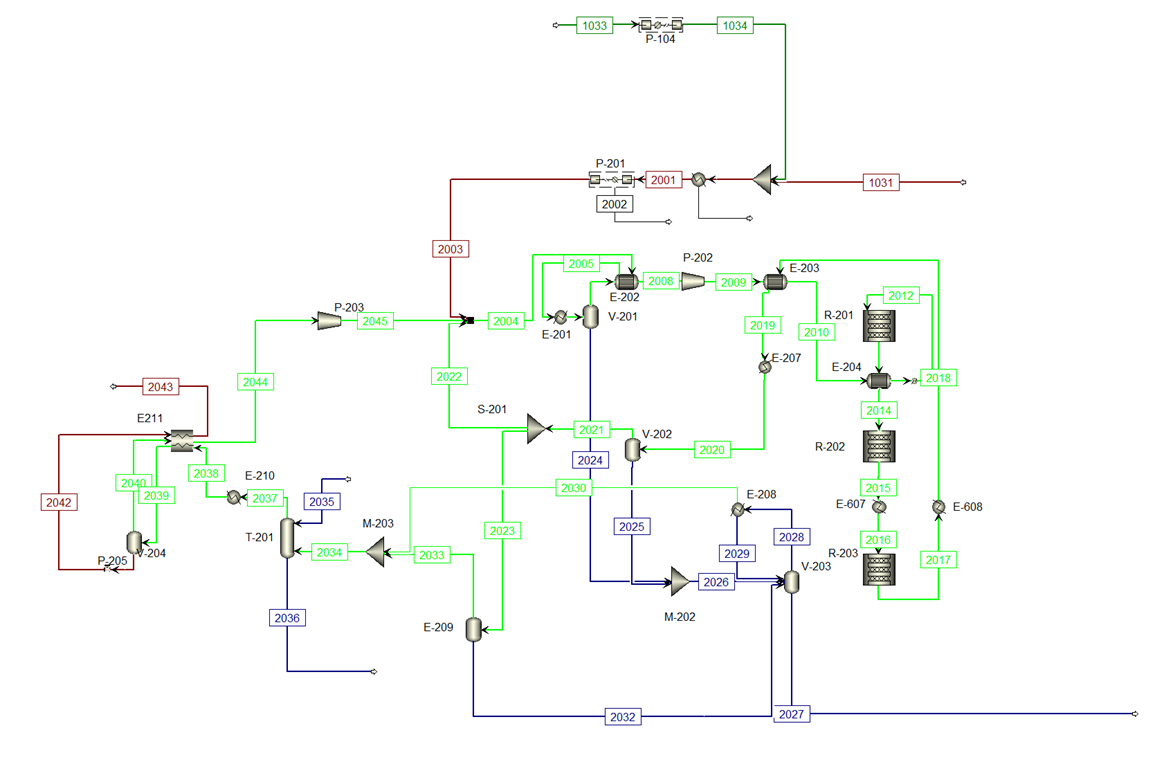
\includegraphics[width=\textwidth]{img/aspen_nh3.png}
	\caption{Ammonia synthesis process flow diagram}
	\label{img_aspennh3}
\end{figure}

Syngas from the gasification and gas conditioning (1031) is mixed with nitrogen from the air separation unit (1033), 
maintaining a molar $H_2/N_2$ ratio of 2.9:1. The syngas is compressed to the process pressure of 200 bar and sent to 
the loop, where it is mixed with the recycle gases (2022) and the rich $H_2$ gas from the purge gas treatment. 
The gas mixture is chilled to -20°C in heat exchangers (E-202 and E-201). The liquid is separated in flash drum 
(V-201), while the gas phase is sent to the circulation compressor (P-202), designed to withstand the pressure loss 
of the system. 

The compressed gases (2009) are sent to the reactor; they are pre-heated to 310°C utilizing the outlet gas from the 
reactor (2018) and first reactor beds (2013), and sent to the first bed. The reactor possesses three catalytic beds, 
R-201/202/203, operating with inlet temperatures of 310°C, 420°C and 380°C. This inlet temperature is maintained by 
indirect intermediate cooling between each bed, to leverage the favorable equilibrium conditions at lower temperatures.
Between the first and second bed, the gas is cooled by the reactor feed, while the heat exchangers E-607 and E-608 cool
the gases by generating steam in the utility plant. 

After all heat recoveries, the reactor outlet stream (2019) is cooled to 30°C with cooling water on E-207. Most of the 
liquid $NH_3$ is recovered on this first cooling stage. The gas phase of separation drum V-202 (2021) is recycled back
into the process, except for a purge fraction (2023) of 3\% of the total loop flow. This purge is designed to keep the
total inert molar fraction in the ammonia loop close to 10\%, as the inerts reduce the reactants conversion and
increase the circulation rate \cite{florez-orregoProcessSynthesisOptimization2018}. 
The liquid $NH_3$ from both condensers (2024, 2025) is expanded to 80 bar to recover a rich $H_2$ stream (2030) and
the final $NH_3$ product (2027) is sent to the urea synthesis unit.

The loop purge gas (2023) contains a about 60\% mol of $H_2$, which is recovered on the cryogenic purge gas treatment 
section. The gas is chilled to -20°C to recover any liquid ammonia not condensed in the main loop and mixed with the
rich $H_2$ gases from the $NH_3$ flashing (2030). The remaining $NH_3$ is removed in the absorber column T-201, 
using water to produce an aqua-ammonia stream (2036). The outlet gases from the absorber (2037) are again cooled to
-20°C  in heat exchanger E-210, and refrigerated to -192°C in the cold box E-211, where the majority of the non-$H_2$
components such as $CH_4$ and $N_2$ condense. The liquid fraction of the outlet mixture is separated in the flash drum V-204 and expanded to atmospheric pressure to drive the inlet gas cooling. The recovered rich $H_2$ stream (2044) is re-compressed
and sent back to the ammonia loop, while the $CH_4$-rich stream (2043) is sent to the utilities plant.

The gas properties for this unit were calculated using the Peng-Robinson equation of state with Boston-Mathias
modifications.

\subsubsection{Urea synthesis}
The urea synthesis consists of the formation of ammonium carbamate, and its dehydration into urea, and can be
represented by the following reactions:

\begin{alignat}{2}
	&2NH_3 + CO_2 \rightleftharpoons NH_4NH_2CO_2 \quad & &\Delta H_{ref}^0 = -117 kJ/mol  \\
	&NH_4NH_2CO_2 \rightleftharpoons (NH_2)_2CO + H_2O \quad & &\Delta H_{ref}^0 = +15.5 kJ/mol 
\end{alignat}

Both reactions occur exclusively in the liquid phase. The carbamate formation is strongly exothermic and fast, while 
the urea formation is slow and slightly endothermic, and is therefore the determining step of the process.




\printbibliography{}


\end{document}
